\chapter{Resultados} \label{results}
En este capítulo se presenta el estado en el que quedó la aplicación eFuel al finalizar el desarrollo. Se completó el 92\% de los casos de uso que tiene el sistema actualmente. No se realizaron pruebas de ningún tipo salvo por demostraciones del funcionamiento en una instalación local, sin embargo, el dueño del producto quedó satisfecho con el trabajo realizado y se espera que el desarrollo continue en el futuro. A continuación se presenta el diagrama de casos de uso y un resumen de la funcionalidad que posee el sistema actualmente. Además, se presentan 2 diagramas para ayudar a describir la estrctura del sistema: modelo de dominio y el diagrama de componentes. Para información detallada del funcionamiento e implementación del sistema referirse al Documento de Arquitectura de Software (anexo \ref{das}).

\section{Casos de Uso} \label{useCases}
En los siguientes diagramas se muestran en color verde los casos de uso que fueron implementados.

\begin{figure}[H]
    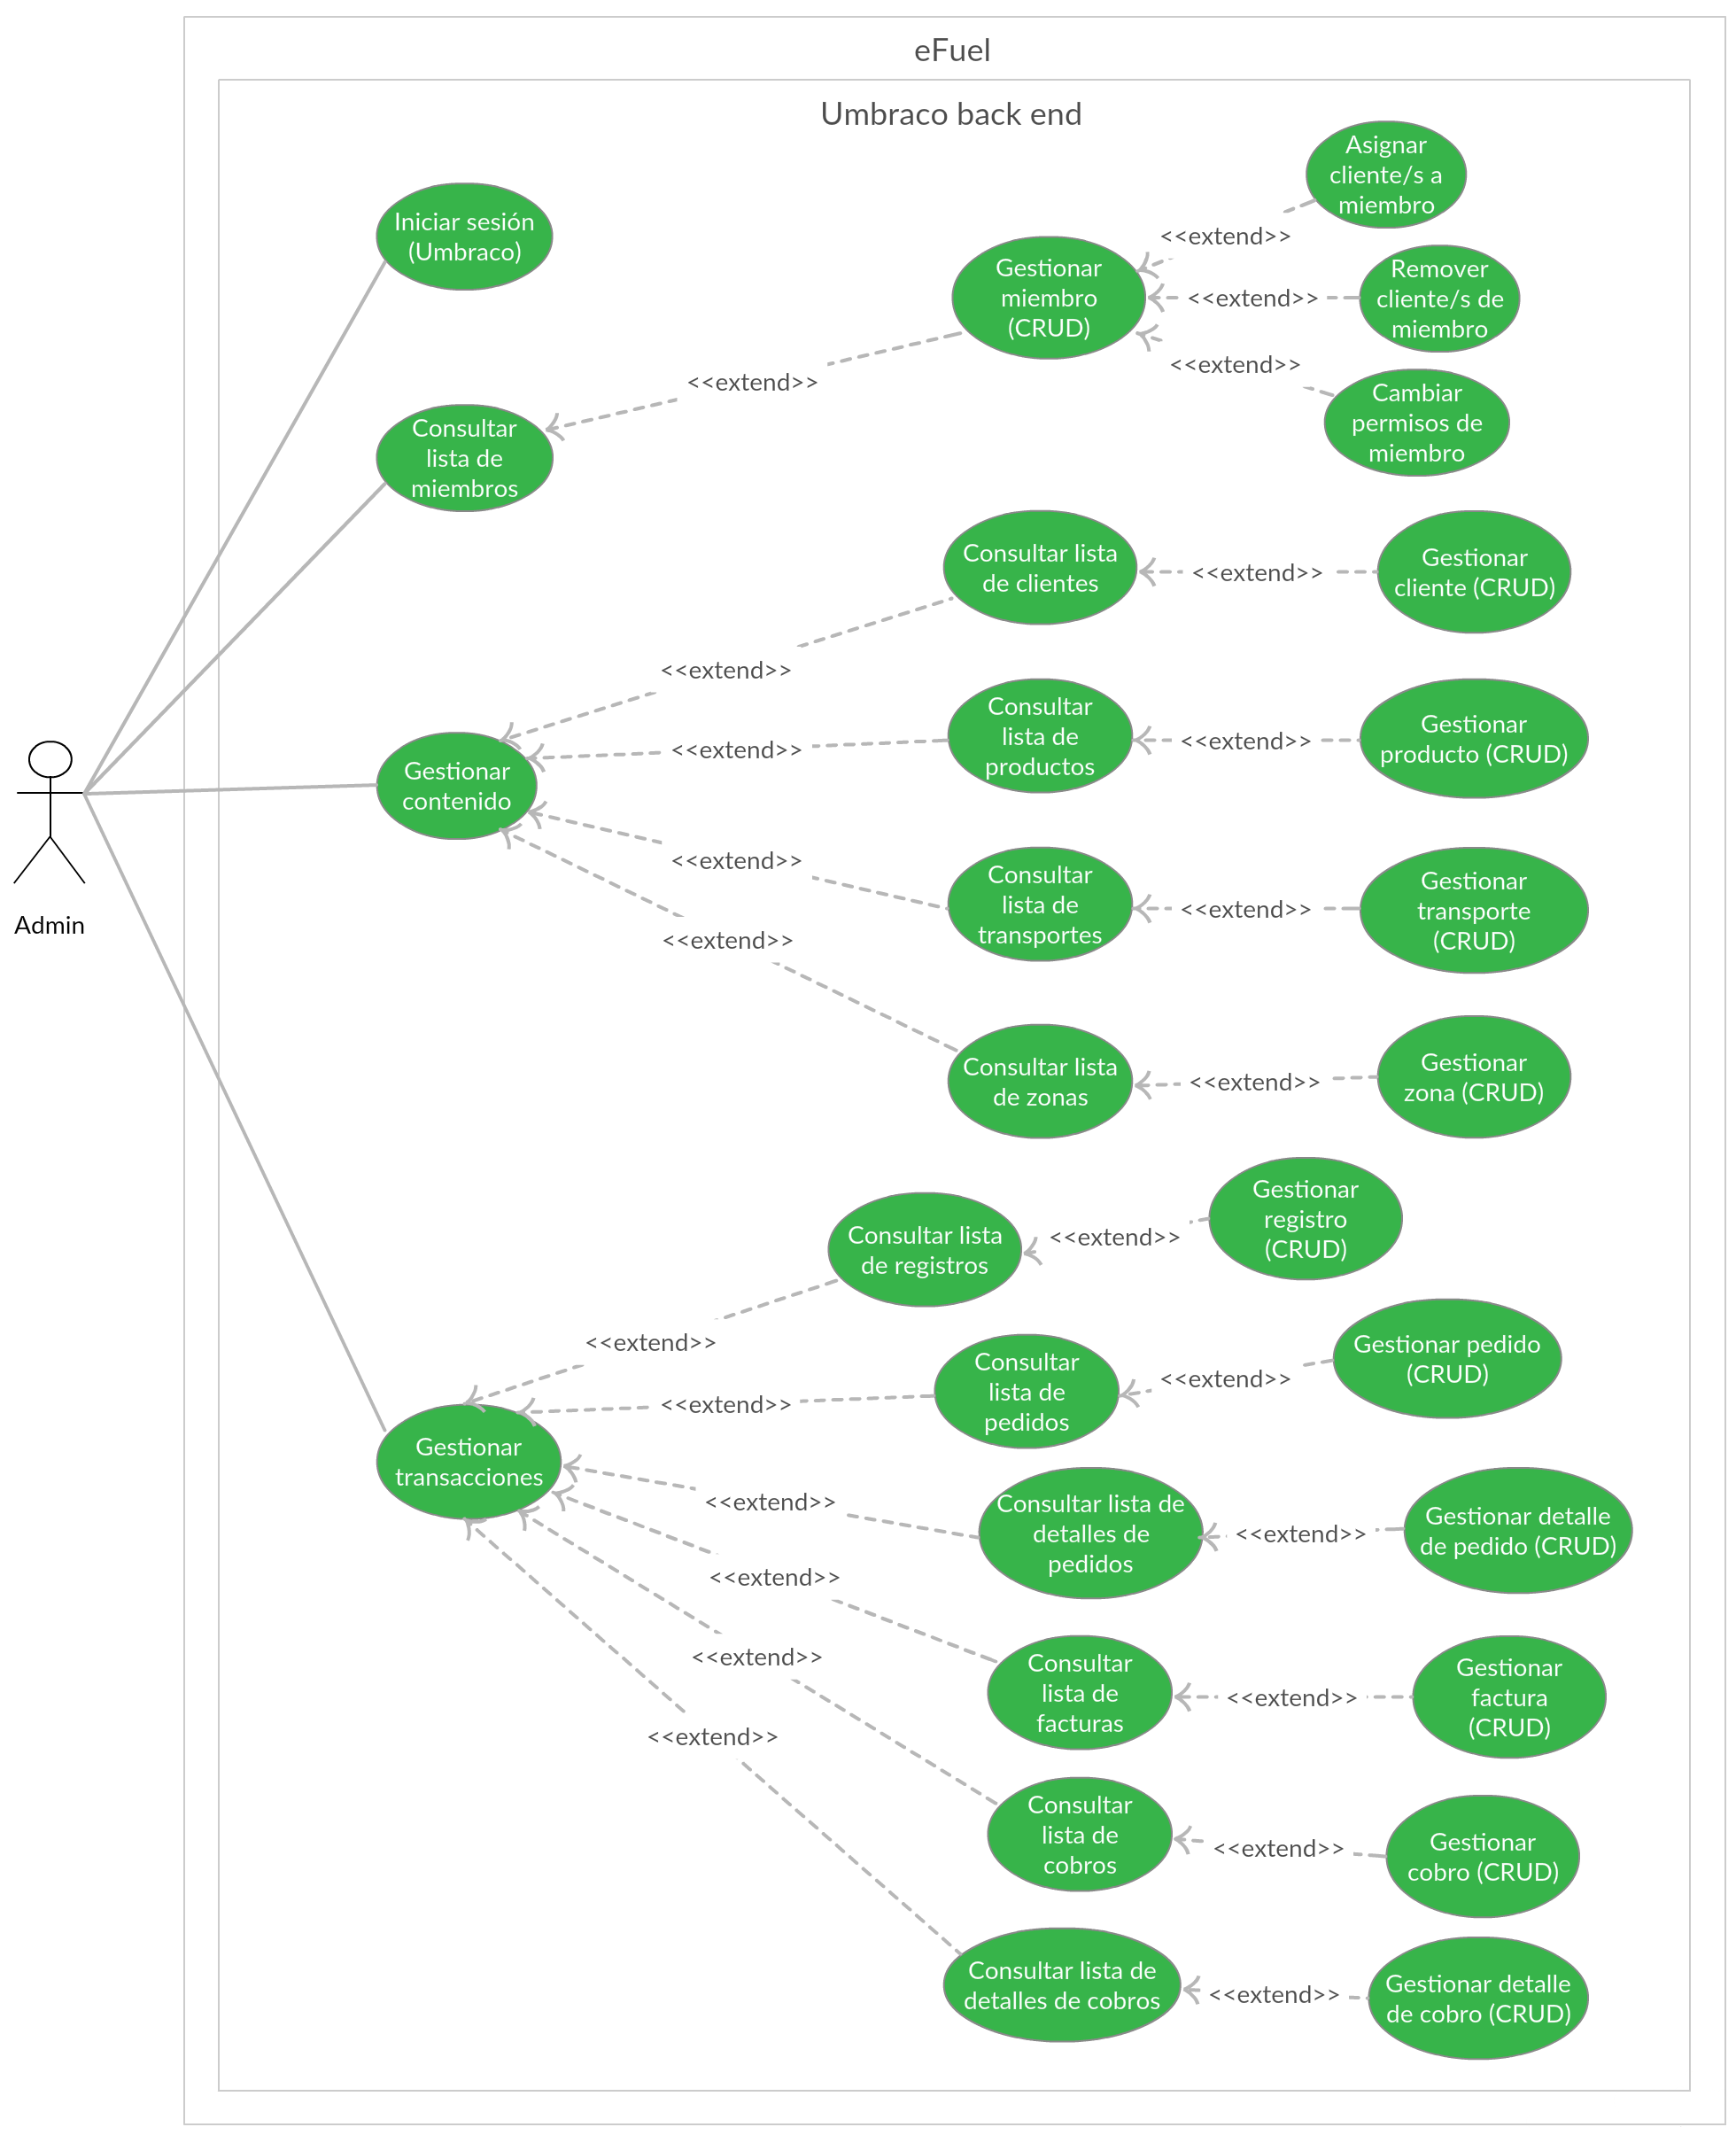
\includegraphics[width=\textwidth]{cu_admin_implementados.png}
    \caption{Casos de Uso back end (\emph{admin})}
    \label{fig:cu_admin_implementados}
    \centering
\end{figure}

\begin{figure}[H]
    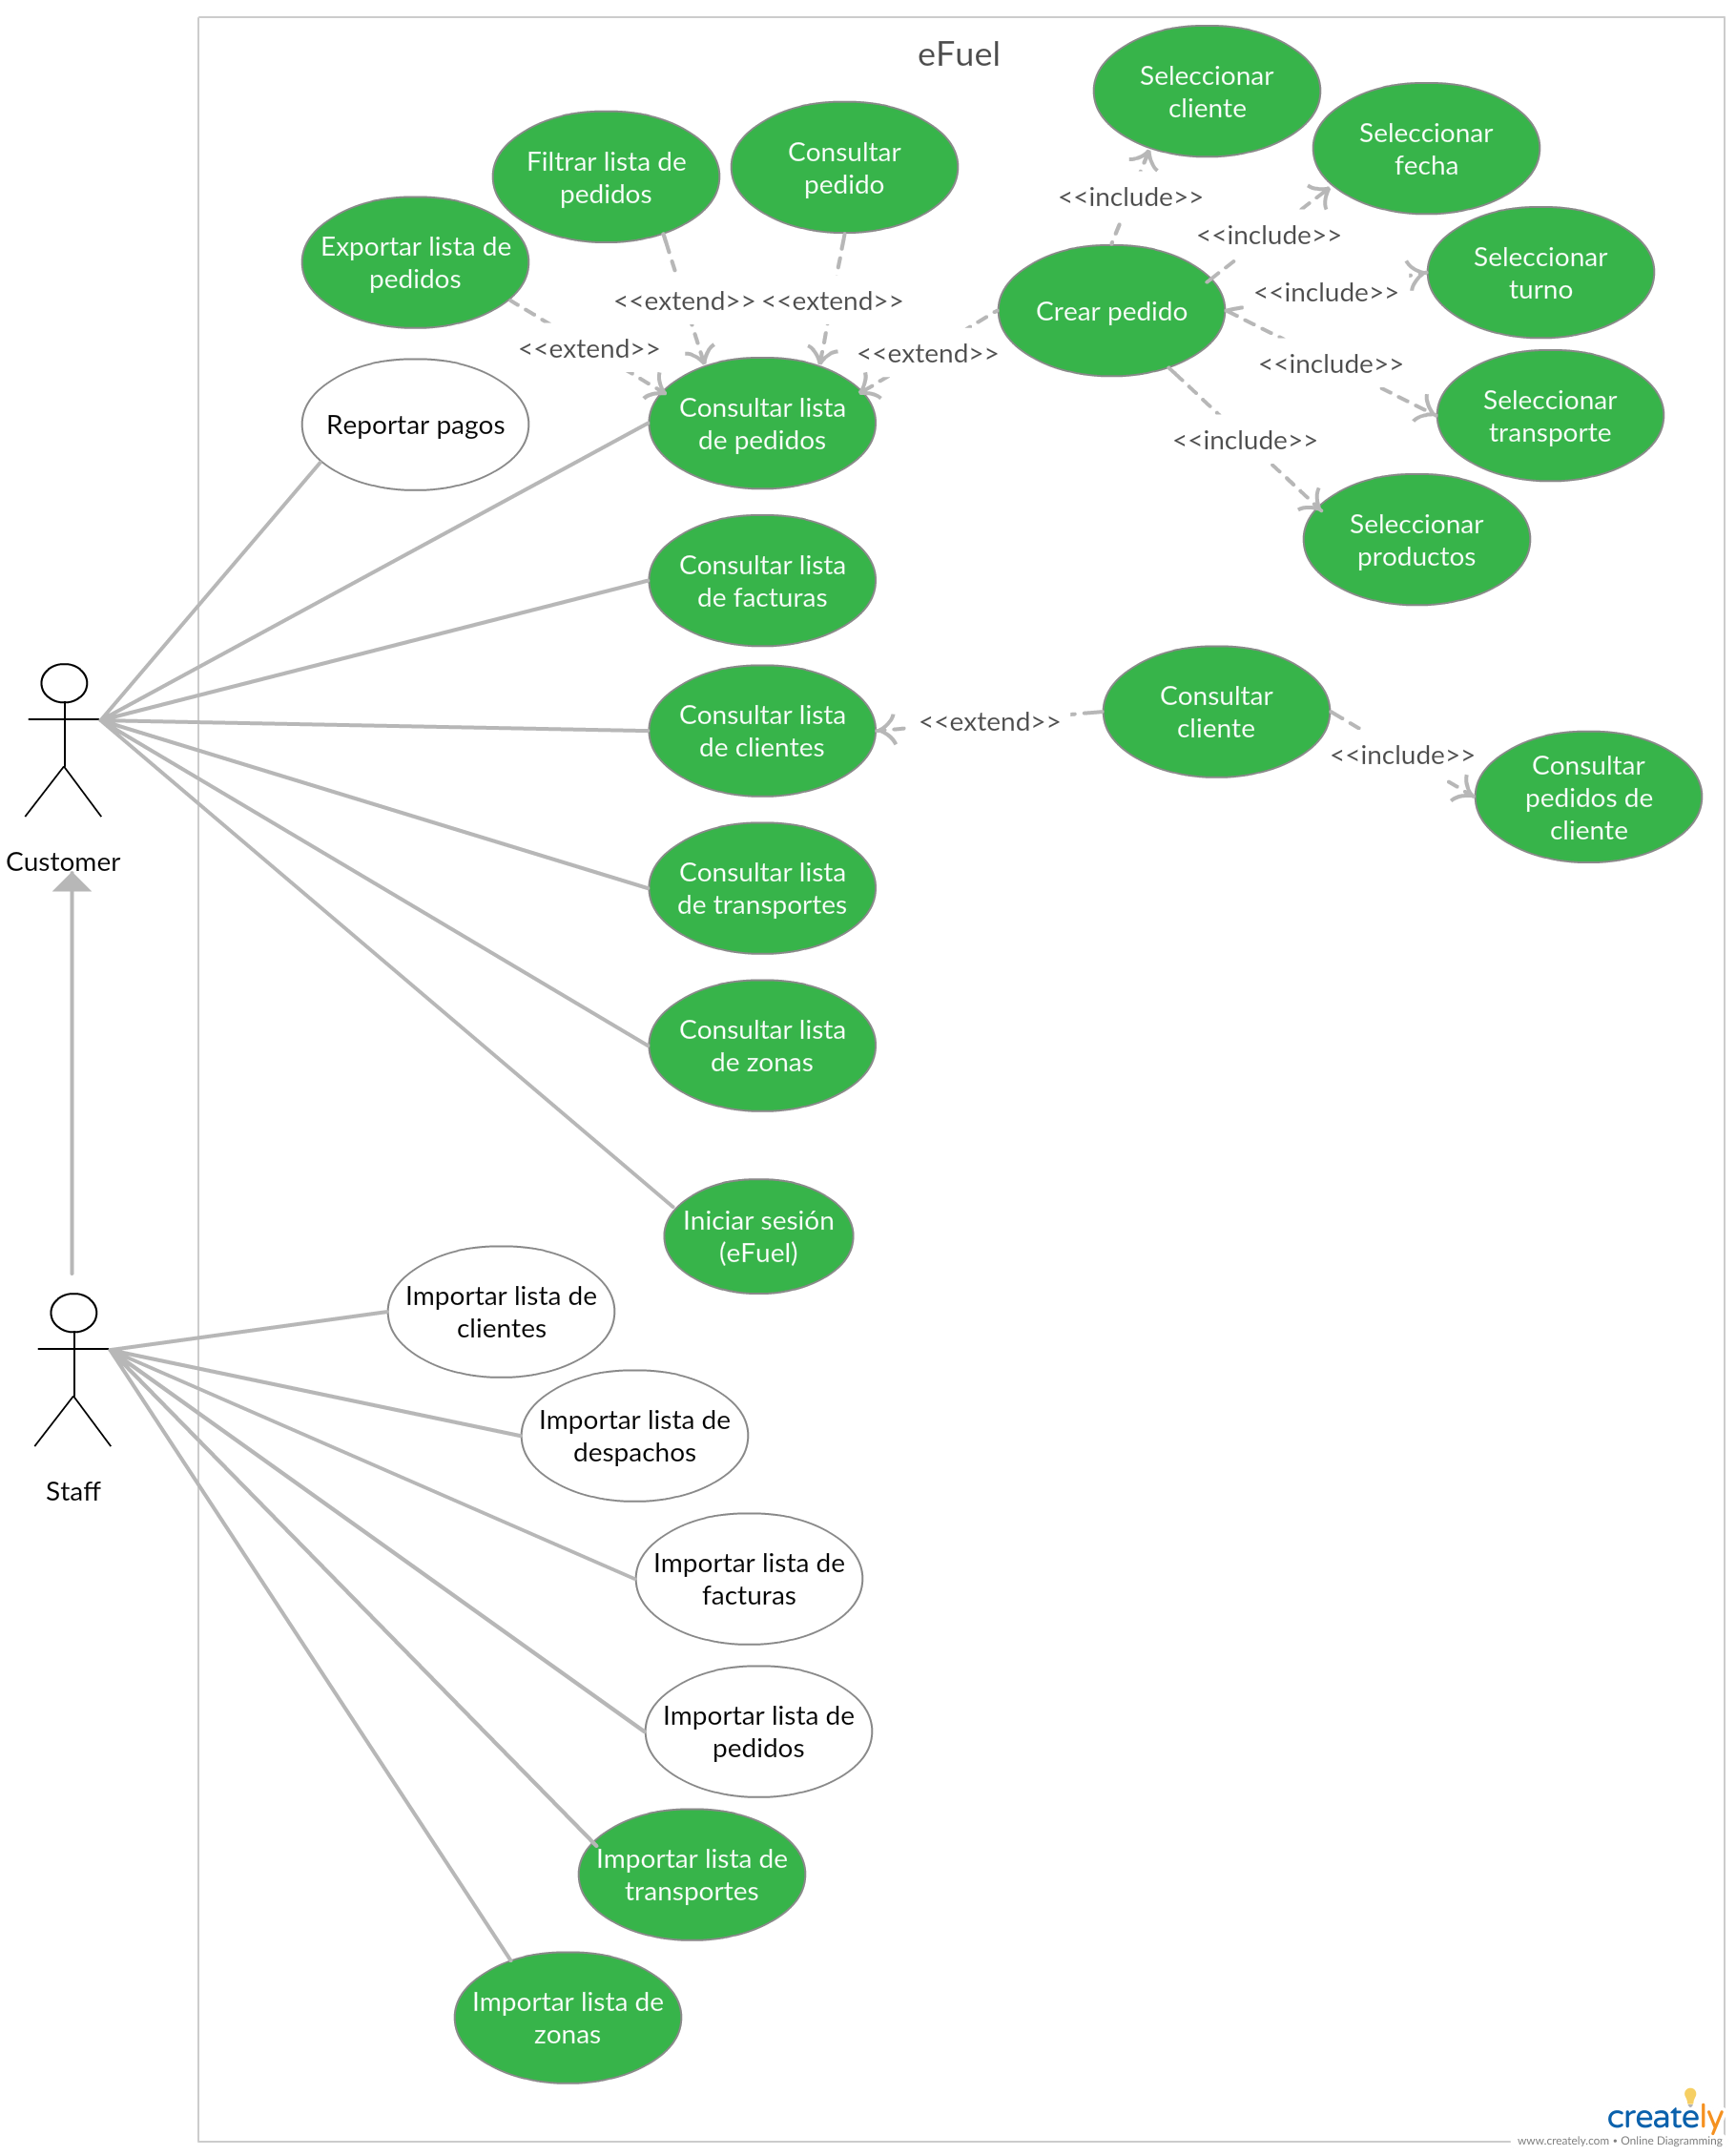
\includegraphics[width=\textwidth]{cu_customer_staff_implementados.png}
    \caption{Casos de Uso front end (\emph{customer} y \emph{staff})}
    \label{fig:cu_customer_staff_implementados}
    \centering
\end{figure}

\section{Estado actual de la aplicación}
Como resultado del desarrollo del proyecto se obtuvo una aplicación web desarrollada nuevamente que funciona como un agregado a un sitio de Umbraco y que contiene, casi en su totalidad, las funcionalidades requeridas por el dueño del producto. No se ha desplegado la aplicación en un ambiente de producción, solo fue probada en varias instalaciones locales, a pesar de esto el dueño del producto quedó satisfecho con los resultados obtenidos. Sigue un resumen de la funcionalidad que tiene la aplicación, dividido en partes: funcionalidad en el front end de eFuel y funcionalidad en el back end de Umbraco.

\subsection{Funcionalidad en el front end}
\begin{itemize}
    \item Creación de pedidos según la disponibilidad de transportes, fechas y turnos para un cliente.
    \item Listado de pedidos con filtros por cliente, rango de fecha, transporte y estado.
    \item Exportación de un listado de pedidos con filtros aplicados.
    \item Visualización de la lista de clientes, transportes, zonas y facturas.
    \item Importación de lista de transportes y zonas.
\end{itemize}

\subsection{Funcionalidad en el back end de Umbraco}
\begin{itemize}
    \item Listado de clientes, transportes, zonas, turnos y productos.
    \item Creación, edición, vista de detalles y eliminación de clientes, transportes, zonas, turnos y productos.
    \item Listado de pedidos, facturas y cobros.
    \item Creación, edición, vista de detalles y eliminación de pedidos, facturas y cobros.
    \item 
\end{itemize}
